\documentclass[11pt,aspectratio=169]{beamer}
\usetheme{default}
\usecolortheme{seagull}
\setbeamertemplate{navigation symbols}{}
\setbeamertemplate{footline}[frame number]
\setbeamertemplate{itemize items}[circle]
\setbeamerfont{frametitle}{size=\large,series=\bfseries}
\setbeamercolor{frametitle}{fg=black}
\setbeamercolor{block title}{bg=black!8,fg=black}
\setbeamercolor{block body}{bg=black!3}
\usepackage{amsmath, amssymb}
\usepackage{tikz}
\usetikzlibrary{arrows.meta, positioning}
\newcommand{\E}{\mathbb{E}}
\newcommand{\dE}{\Delta E}
\newcommand{\dP}{\Delta P}
\newcommand{\calA}{\mathcal{A}}
\newcommand{\sg}{\mathrm{sg}}
\newcommand{\gray}[1]{{\color{black!55}#1}}

\title{Constructing sufficient agent states\\ from plasticity and empowerment}
\author{Zihan Wang}
\date{October 2026}

\begin{document}

\begin{frame}
\titlepage
\begin{center}\small\gray{Can an agent build a state from its own stream, and do plasticity and empowerment help?}\end{center}
\end{frame}

% ---------------------------------------------------------------
\begin{frame}{The agent keeps a memory and acts from it}
\begin{center}
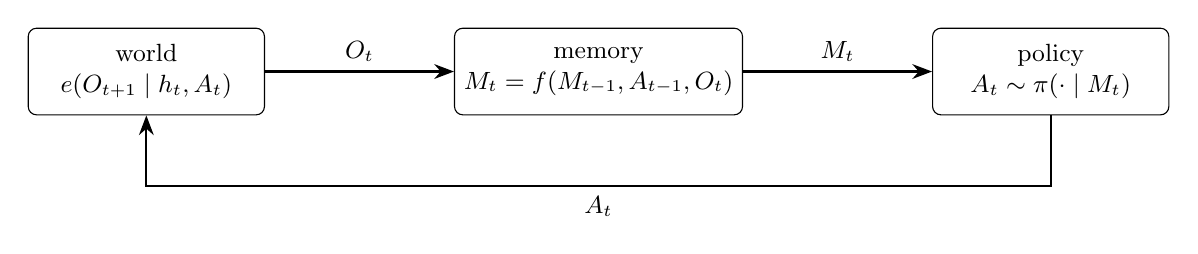
\begin{tikzpicture}[>={Stealth[length=2.5mm]}, node distance=14mm and 24mm,
  box/.style={draw, rounded corners=3pt, minimum height=11mm, minimum width=30mm, align=center, font=\small}]
\node[box] (world) {world\\ $e(O_{t+1}\mid h_t, A_t)$};
\node[box, right=of world] (mem) {memory\\ $M_t = f(M_{t-1}, A_{t-1}, O_t)$};
\node[box, right=of mem] (pol) {policy\\ $A_t \sim \pi(\cdot \mid M_t)$};
\draw[->, thick] (world) -- node[above, font=\small] {$O_t$} (mem);
\draw[->, thick] (mem) -- node[above, font=\small] {$M_t$} (pol);
\draw[->, thick] (pol.south) -- ++(0,-9mm) -| node[pos=0.25, below, font=\small] {$A_t$} (world.south);
\end{tikzpicture}
\end{center}
\vspace{2mm}
\begin{itemize}
\item History $h_t = (O_{1:t}, A_{1:t-1})$. The reward is one component of $O_t$.
\item The world may depend on the whole history. No Markov assumption. A changing world is one such law.
\item The memory is a function of the history, $M_t = \phi_t(h_t)$; the action depends on $h_t$ only through $M_t$.
\end{itemize}
\vspace{2mm}
\textbf{Question.} When is the memory \emph{enough}?
\end{frame}

% ---------------------------------------------------------------
\begin{frame}{``Enough'' is one number}
\begin{block}{State defect}
\[
D_t \;=\; I\big(h_t;\, O_{t+1} \,\big|\, M_t, A_t\big)
\]
\end{block}
\vspace{1mm}
In words: once you know the memory and the action, how much does the history still tell you about what comes next?
\vspace{3mm}
\begin{itemize}
\item $D_t = 0$ \;$\Longleftrightarrow$\; two histories with the same memory give the same law of $O_{t+1}$, for every action the agent takes.
\item Then we call $M$ a \textbf{sufficient predictive state}.
\item It is a statement about the pairs $(h_t, a)$ that actually occur, not about all histories and actions.
\end{itemize}
\end{frame}

% ---------------------------------------------------------------
\begin{frame}{Why $D_t = 0$ gives the best return}
\begin{enumerate}
\item The reward is inside $O_{t+1}$, and $M_{t+1} = f(M_t, A_t, O_{t+1})$.\\
  So if $O_{t+1}$ does not depend on $h_t$ given $(M_t, A_t)$, neither does $(R_{t+1}, M_{t+1})$:
  \[
  \Pr(R_{t+1}, M_{t+1} \mid h_t, A_t) = \Pr(R_{t+1}, M_{t+1} \mid M_t, A_t) .
  \]
\item So (reward, next memory) is a Markov decision process on memory values. Bellman on memory, time by time:
  \[
  q^*_t(m, a) = \sum_{r, m'} \Pr(r, m' \mid m, a)\,[\,r + \gamma\, v^*_{t+1}(m')\,], \qquad v^*_t(m) = \max_{a \text{ taken at } m} q^*_t(m, a).
  \]
\item $v^*_t(M_t)$ is the best return over \emph{all} behaviours that use the actions the agent takes; if every action keeps positive probability, $q^*_t(M_t, a) = Q^*_t(h_t, a)$ and greedy on $q^*$ is optimal.
\end{enumerate}
\vspace{2mm}
\gray{Existence only: an optimal policy reading $M_t$ exists. Whether PPO finds it is a different question.}
\end{frame}

% ---------------------------------------------------------------
\begin{frame}{One example before the theory: matching pennies}
A fair coin is shown. Reward $1$ if the action matches it. Uniform policy.
\vspace{2mm}
\begin{center}\small
\begin{tabular}{lcc}
 & memory $=$ nothing & memory $=$ the coin \\ \hline
predicts the stream without the action & perfectly (two fair coins) & perfectly \\
knows what the action does to the reward & no & yes \\
$D_t$ & $1$ bit & $0$ \\
\end{tabular}
\end{center}
\vspace{3mm}
\textbf{Lesson.} A memory can predict everything it will see and still be useless for control.\\
The missing bit is exactly the \emph{empowerment} the memory fails to see. The rest of the talk makes this exact.
\end{frame}

% ---------------------------------------------------------------
\begin{frame}{Abel's two flows, read in two places}
\begin{columns}
\column{0.5\textwidth}
\textbf{Empowerment}: the action changes what comes next
\[
E_t = I(A_t;\, O_{t+1} \mid h_t)
\]
read from the memory instead of the history:
\[
E_t(M) = I(A_t;\, O_{t+1} \mid M_t)
\]
\column{0.5\textwidth}
\textbf{Plasticity}: the new observation changes the next action
\[
P_{t+1} = I(O_{t+1};\, A_{t+1} \mid h_t, A_t)
\]
read from the memory:
\[
P_{t+1}(M) = I(O_{t+1};\, A_{t+1} \mid M_t, A_t)
\]
\end{columns}
\vspace{4mm}
\begin{itemize}
\item Nothing new is defined: the second row is the first with the history replaced by the memory.
\item The agent can only compute the memory versions. The history versions are the ideal.
\item We never ask for a large or small amount of either. We ask: \textbf{how much does the memory misread them?}
\end{itemize}
\end{frame}

% ---------------------------------------------------------------
\begin{frame}{Empowerment mismatch, every step}
Write each information as a difference of two entropies:
\begin{align*}
E_t &= H(A_t \mid h_t) \;-\; H(A_t \mid h_t, O_{t+1}) \\
E_t(M) &= H(A_t \mid M_t) \;-\; H(A_t \mid M_t, O_{t+1})
\end{align*}
The action depends on the history only through the memory, so
\[
H(A_t \mid h_t) = H(A_t \mid M_t) .
\]
Subtract; the first terms cancel:
\[
\dE_t \;=\; E_t - E_t(M) \;=\; H(A_t \mid M_t, O_{t+1}) - H(A_t \mid h_t, O_{t+1}) .
\]
Because $M_t$ is a function of $h_t$, conditioning on $h_t$ is conditioning on $(h_t, M_t)$, so the difference is a mutual information:
\[
\boxed{\;\dE_t = I(h_t;\, A_t \mid M_t, O_{t+1}) \;\ge\; 0\;}
\]
\textbf{Meaning.} Once the result is seen, the forgotten history still explains the action. A memory can only \emph{under}-read empowerment.
\end{frame}

% ---------------------------------------------------------------
\begin{frame}{Plasticity mismatch, every step}
Four entropy terms:
\begin{align*}
P_{t+1} &= H(A_{t+1} \mid h_t, A_t) \;-\; H(A_{t+1} \mid h_t, A_t, O_{t+1}) \\
P_{t+1}(M) &= H(A_{t+1} \mid M_t, A_t) \;-\; H(A_{t+1} \mid M_t, A_t, O_{t+1})
\end{align*}
Both second terms are the same number, $H(A_{t+1} \mid M_{t+1})$:
\begin{itemize}
\item $(h_t, A_t, O_{t+1}) = h_{t+1}$, and the next action depends on $h_{t+1}$ only through $M_{t+1}$;
\item $(M_t, A_t, O_{t+1})$ determines $M_{t+1} = f(M_t, A_t, O_{t+1})$, and the next action depends only on $M_{t+1}$.
\end{itemize}
Subtract; the second terms cancel:
\begin{align*}
\dP_t \;=\; P_{t+1}(M) - P_{t+1} &\;=\; H(A_{t+1} \mid M_t, A_t) - H(A_{t+1} \mid h_t, A_t) \\
&\;=\; \boxed{\; I(h_t;\, A_{t+1} \mid M_t, A_t) \;\ge\; 0 \;}
\end{align*}
\textbf{Meaning.} The forgotten history still predicts the agent's own next move. A memory can only \emph{over}-read plasticity.
\end{frame}

% ---------------------------------------------------------------
\begin{frame}{The decomposition, every step}
Take the information that history and action together carry about what comes next, beyond the memory, and expand it in both orders.
\begin{align*}
I(h_t, A_t;\, O_{t+1} \mid M_t) &= \underbrace{I(h_t; O_{t+1} \mid M_t)}_{D^0_t\ \text{(prediction without the action)}} + \underbrace{I(A_t; O_{t+1} \mid M_t, h_t)}_{=\,E_t\ \text{(given $h_t$, $M_t$ adds nothing)}} \\[1mm]
I(h_t, A_t;\, O_{t+1} \mid M_t) &= \underbrace{I(A_t; O_{t+1} \mid M_t)}_{E_t(M)} + \underbrace{I(h_t; O_{t+1} \mid M_t, A_t)}_{D_t}
\end{align*}
Equate the two right-hand sides, $D^0_t + E_t = E_t(M) + D_t$:
\[
\boxed{\;D_t \;=\; D^0_t \;+\; \dE_t\;}
\]
For plasticity: given $(M_t, A_t)$, $h_t \to O_{t+1} \to M_{t+1} \to A_{t+1}$ is a chain, so by data processing
\[
\boxed{\;0 \;\le\; \dP_t \;\le\; D_t\;}
\]
\end{frame}

% ---------------------------------------------------------------
\begin{frame}{What the two boxes say}
\begin{block}{A memory is a sufficient predictive state if and only if}
it predicts the next observation as well as the history does \emph{without} the action \;($D^0_t = 0$)\\
\textbf{and} it loses no empowerment \;($\dE_t = 0$).
\end{block}
\vspace{2mm}
\begin{itemize}
\item Empowerment is the half of the defect that action-free prediction cannot see.\\ Pennies, constant memory: $D^0_t = 0$, $\dE_t = D_t = 1$ bit.
\item Plasticity is not a third half. It is a \textbf{lower bound}: an excess read from the agent's own next move proves something was forgotten. It needs no model of the world.
\item Plasticity alone cannot certify a state: a policy that ignores its memory has $\dP_t = 0$ for every memory (pennies again: $\dP_t = 0$, $D_t = 1$ bit).
\end{itemize}
\end{frame}

% ---------------------------------------------------------------
\begin{frame}{From the whole history to a window the agent can keep}
During training the agent keeps a window of its own trajectory, $W_t = (O_{t-k:t}, A_{t-k:t-1})$, and compares $M_t$ with $M^+_t = (M_t, W_t)$.
\begin{align*}
L^*_O &= H(O_{t+1} \mid M_t) - H(O_{t+1} \mid M^+_t) && \text{how much the window helps predict} \\
L^*_E &= H(A_t \mid M_t, O_{t+1}) - H(A_t \mid M^+_t, O_{t+1}) && \text{how much it helps the inverse model} \\
L^*_P &= H(A_{t+1} \mid M_t, A_t) - H(A_{t+1} \mid M^+_t, A_t) && \text{how much it helps predict the next action}
\end{align*}
Same chain rules with $W_t$ in place of $h_t$:
\begin{align*}
L^*_O + L^*_E &= I(W_t; O_{t+1} \mid M_t, A_t) =: D^{(k)}_t, \qquad 0 \le L^*_P \le D^{(k)}_t \le D_t, \\
D_t - D^{(k)}_t &= I(h_t;\, O_{t+1} \mid M_t, A_t, W_t).
\end{align*}
\vspace{1mm}
\textbf{The residual is what lies outside the window.} Reward that follows the action taken three steps ago, window of one step, constant memory: all window losses are $0$, yet $D_t = 1$ bit.\\
\gray{Zero window mismatch does not certify a state. Nothing computed from finite interaction can.}
\end{frame}

% ---------------------------------------------------------------
\begin{frame}[shrink=12]{The algorithm, in one picture}
\begin{center}
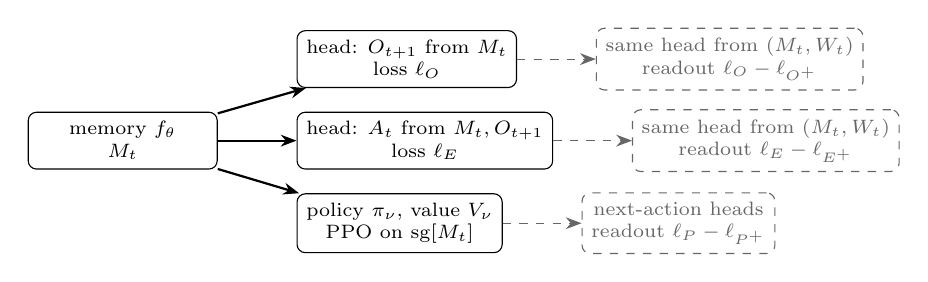
\begin{tikzpicture}[>={Stealth[length=2mm]}, node distance=3mm and 10mm,
  box/.style={draw, rounded corners=3pt, minimum height=7mm, minimum width=24mm, align=center, font=\scriptsize},
  dim/.style={box, dashed, draw=black!60, text=black!60}]
\node[box] (mem) {memory $f_\theta$\\ $M_t$};
\node[box, above right=of mem] (ho) {head: $O_{t+1}$ from $M_t$\\ loss $\ell_O$};
\node[box, right=of mem] (he) {head: $A_t$ from $M_t, O_{t+1}$\\ loss $\ell_E$};
\node[box, below right=of mem] (pi) {policy $\pi_\nu$, value $V_\nu$\\ PPO on $\sg[M_t]$};
\node[dim, right=of ho] (hop) {same head from $(M_t, W_t)$\\ readout $\ell_O - \ell_{O^+}$};
\node[dim, right=of he] (hep) {same head from $(M_t, W_t)$\\ readout $\ell_E - \ell_{E^+}$};
\node[dim, right=of pi] (hp) {next-action heads\\ readout $\ell_P - \ell_{P^+}$};
\draw[->, thick] (mem) -- (ho); \draw[->, thick] (mem) -- (he); \draw[->, thick] (mem) -- (pi);
\draw[->, dashed, black!60] (ho) -- (hop); \draw[->, dashed, black!60] (he) -- (hep); \draw[->, dashed, black!60] (pi) -- (hp);
\end{tikzpicture}
\end{center}
\begin{itemize}\small
\item The memory learns from $\ell_O + \lambda\,\ell_E$, the two halves of the defect; the policy never shapes the memory.
\item The dashed heads see a longer window; their differences estimate $L^*_O, L^*_E, L^*_P$ and change no gradient: readouts.
\item Honest consequence: the memory objective is ordinary prediction; the theory says \emph{what} it does, and adds two readouts.
\end{itemize}
\end{frame}

% ---------------------------------------------------------------
\begin{frame}{Proved, and open}
\begin{columns}[T]
\column{0.5\textwidth}
\textbf{Proved}
\begin{itemize}
\item $D_t = 0$ $\Rightarrow$ Bellman on memory is exact; optimal when every action is tried.
\item $\dE_t = I(h_t; A_t \mid M_t, O_{t+1}) \ge 0$, \; $\dP_t = I(h_t; A_{t+1} \mid M_t, A_t) \ge 0$.
\item $D_t = D^0_t + \dE_t$, \; $0 \le \dP_t \le D_t$.
\item Window versions: same identities; the residual is what the window cannot see.
\item Action-conditioned prediction already targets $D_t$; the memory loss of the algorithm equals it on the data, up to an inertia term.
\end{itemize}
\column{0.5\textwidth}
\textbf{Open}
\begin{itemize}
\item Does training actually reach $D_t = 0$?
\item Do the readouts track the gaps with finite data and imperfect heads?
\item Do the inverse and next-action heads help beyond one action-conditioned predictor? (Test on worlds where both halves are known exactly.)
\item How fast does the memory recover after the world changes?
\end{itemize}
\end{columns}
\vspace{4mm}
\begin{center}
\textbf{One line.} Information-flow mismatches characterise a sufficient state and give candidate training signals; whether they beat plain prediction in continual RL is the question to test.
\end{center}
\end{frame}

\end{document}
